\section{QAOA Setup Summary}

The methodological choices adopted throughout this chapter can be summarized as follows:
\begin{itemize}
    \item \textbf{Layer-by-layer training:} QAOA parameters are optimized incrementally, starting from $p=1$ and using previously optimized parameters as initialization for deeper circuits.  
    \item \textbf{Parameter initialization:} New layers are initialized using the heuristic 
    $\gamma_{p+1} \leftarrow \widetilde{\gamma}_p$, $\beta_{p+1} \leftarrow 0$, which outperforms interpolation strategies.  
    \item \textbf{Classical optimizer:} The gradient-based, unbounded BFGS method is employed, providing superior convergence compared to bounded alternatives.  
\end{itemize}

Together, these decisions define a robust and fair QAOA implementation, enabling meaningful comparisons between different problem Hamiltonians and protocols.

\begin{figure}[h]
    \centering
    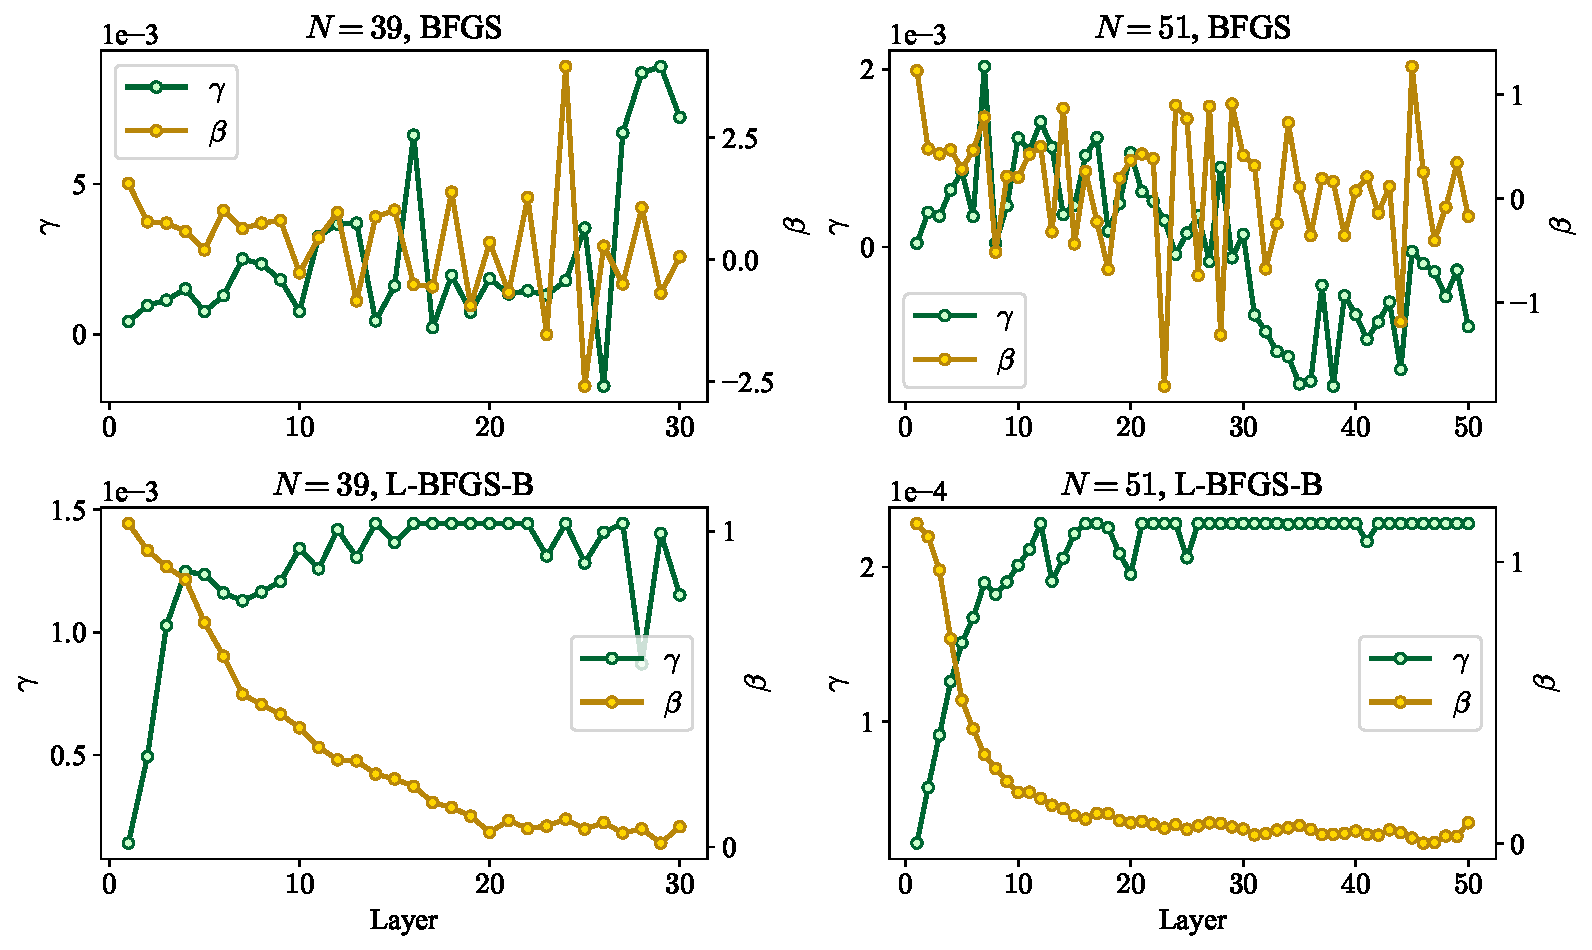
\includegraphics[width=1\textwidth]{03-methodology/figs/optimizer_parameters_comparison.pdf}
    \caption{Variational parameter evolution for $N=39$ and $N=51$ using BFGS and L-BFGS-B. An adiabatic-like trajectory emerges under L-BFGS-B due to parameter bounds.}
    \label{fig:optimizer_parameter_comparison}
\end{figure}